\documentclass{article}
\usepackage[a4paper, paperwidth=25cm, paperheight=25.5cm, left=1.5cm, right=1.5cm, top=1cm, bottom=2cm]{geometry}
\usepackage{tikz,tcolorbox}
\usepackage{amsmath}
\usepackage[table,xcdraw]{xcolor}
\usepackage{listings}
\usepackage{array,multirow} % For customizing tables
\usepackage{booktabs} % For better horizontal lines
\usepackage{makecell}
\setlength{\parindent}{0pt}

\lstset{
    language=SQL,                    % Set language to SQL
    basicstyle=\ttfamily\small,      % Font size and family for code
    keywordstyle=\color{blue}\bfseries, % Color for SQL keywords
    commentstyle=\color{gray},       % Color for comments
    stringstyle=\color{red},         % Color for strings
    numbers=left,                    % Show line numbers on the left
    numberstyle=\tiny\color{gray},   % Line number font and color
    stepnumber=1,                    % Line number step
    breaklines=true,                 % Wrap long lines
    frame=single,                    % Add a frame around code
    tabsize=2,                       % Set tab size
    showstringspaces=false           % Hide spaces in strings
}



\newcommand{\tit}[1]{
\begin{center}
    \Large{\textbf{{#1}}}
\end{center}
}

\definecolor{commentgray}{HTML}{676160}
\definecolor{messagegreen}{HTML}{17B867}
\definecolor{myblue}{HTML}{10C2C4}

\tcbuselibrary{skins, breakable, theorems}


\newtcolorbox{prettyBox}[2]{
  enhanced,
  colback=white!90!#2,   % Background color based on the second parameter (color)
  colframe=#2!60!black,  % Frame color based on the second parameter (color)
  coltitle=white,        % Title color (white)
  fonttitle=\bfseries\Large,
  title=#1,              % Title from the first parameter
  boxrule=1mm,
  arc=0.5mm,
  drop shadow=#2!35!gray, % Drop shadow color based on the second parameter (color)
}



\begin{document}
\tit{TP N\(^{\boldsymbol{\circ}}\)\hspace{0.1cm}3-Les Functions/Procedure}


\vspace{0.75cm}

The includes needed
\begin{itemize}
    \item stdio.h : to printf and get user input
    \item stdlib.h : to use exit to terminate whole 
programe and to terminate child process
    \item unistd.h :to use fork and pipe primitive
    \item ctype.h : to use toupper function
    \item sys/wait.h : to use wait primitive (parent wait for child to terminate)
\end{itemize}
\newpage
\lstinputlisting[style=cstyle,basicstyle=\footnotesize\ttfamily]{Questions/EX1/ex1Overview.c}

child\_1 void function :
\lstinputlisting[style=cstyle,firstline=10,lastline=33,basicstyle=\footnotesize\ttfamily]{Questions/EX1/ex1.c}

\vspace{0.5cm}

child\_2 void function :
\lstinputlisting[style=cstyle,firstline=36,lastline=50,basicstyle=\footnotesize\ttfamily]{Questions/EX1/ex1.c}



\begin{center}
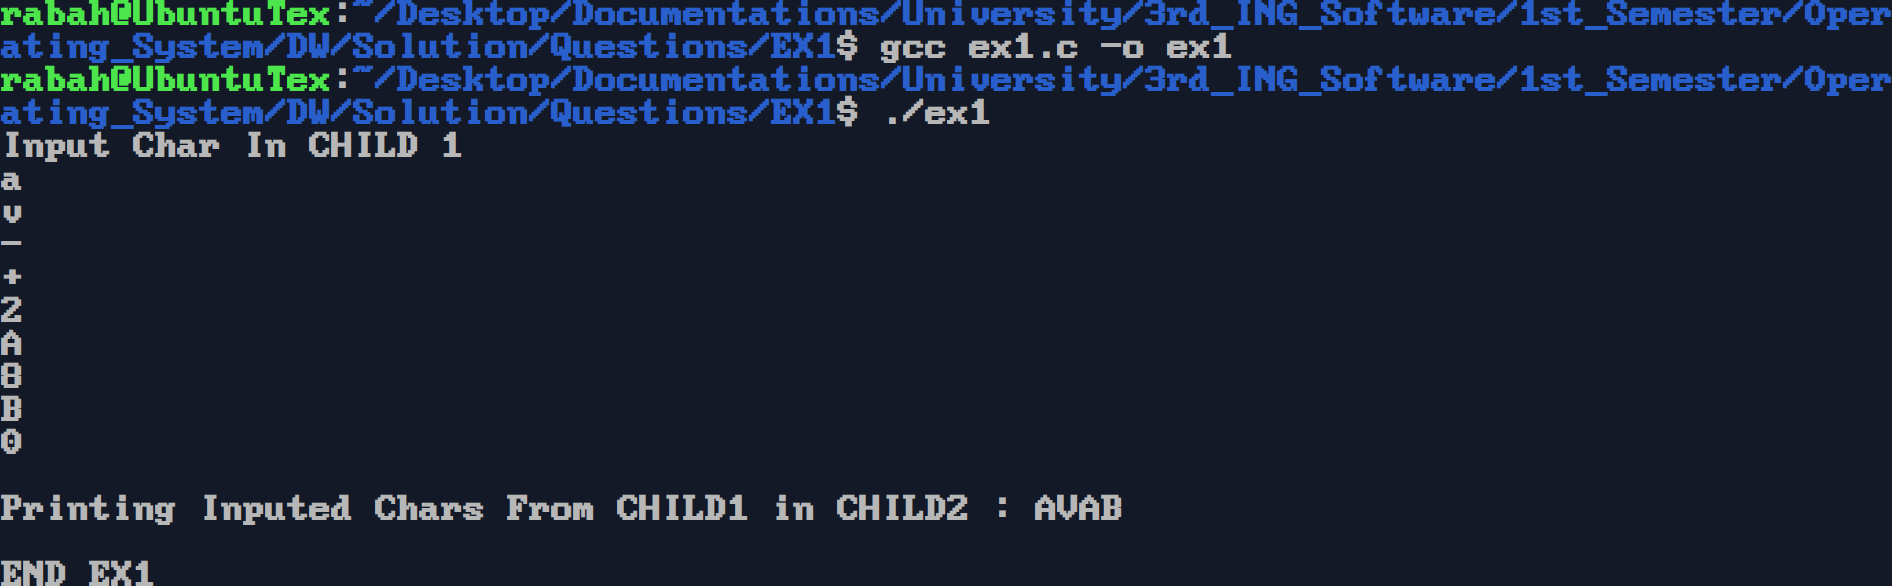
\includegraphics[width=\textwidth]{Questions/EX1/output.png}
\end{center}


\subsubsection*{\underline{Experimental}}
\begin{tabular}{|c|c|c|c|c|c|c|c|c|c|c|c|c|c|c|}
    \hline
    N & \(10^3\) & \(2.10^3\) & \(10^4\) & \(2.10^4\) & \(10^5\) & \(2.10^5\) & \(10^6\) & \(2.10^6\) & \(10^7\) & \(2.10^7\) & \(10^8\) & \(2.10^8\) & \(10^9\) & \(2.10^9\) \\
    \hline
    \makecell{Time\\\((10^{-5})\)} & 8 & 9.8 & 10.8 & 19.4 & 33.6 & 59.3 & 261.1 & 505.7 & 2458.4 & 5071.6 & 24458.7 & 48759.0 & 243312.2 & 487828.6 \\
    \hline
\end{tabular}



\vspace{1cm}

\newpage

\subsubsection*{\underline{Theoritical}}
We first need to find  \(\Delta t\) , for that we will take one runtime value from the experimental study and solve a simple equation 

\vspace{0.15cm}

for n = \(10^4\) and execution time T(n) = \(10.8\times10^{-5}\) :

\vspace{0.75cm}
\begin{align*}
&f(n)\times\Delta t = T(n)\\[0.15cm]
&\Delta t = \frac{T(n)}{f(n)} \\[0.15cm]
&\Delta t = \frac{T(n)}{5n + 6}\\[0.15cm]
&\Delta t = \frac{10.8\times10^{-5}}{5\times 10^4 + 6} \\[0.15cm]
&\Delta t = 2.1597408311\times10^{-9} \\[0.25cm]
&\boxed{\Delta t \approx 2.16\times10^{-9}}
\end{align*}





\vspace{2cm}
\begin{tabular}{|c|c|c|c|c|c|c|c|c|c|c|c|c|c|c|c|c|}
    \hline
    N & \(10^3\) & \(2.10^3\) & \(10^4\) & \(2.10^4\) & \(10^5\) & \(2.10^5\) & \(10^6\) & \(2.10^6\) & \(10^7\) & \(2.10^7\) & \(10^8\) & \(2.10^8\) & \(10^9\) & \(2.10^9\) & \(10^{10}\) & \(2.10^{10}\) \\
    \hline
    \makecell{Time\\\((10^{-5})\)} & 1.08 & 2.16 & 10.08 & 21.6 & 108 & 216 & 1080 & 2160 & 10800 & 21600 & \makecell{108\\\(\times10^3\)} & \makecell{216\\\(\times10^3\)} & \makecell{108\\\(\times10^4\)} & \makecell{216\\\(\times10^4\)} & \makecell{108\\\(\times10^5\)} & \makecell{216\\\(\times10^5\)}\\
    \hline
\end{tabular}

\lstinputlisting[style=cstyle]{Questions/Part4/prime4.c}

\subsubsection*{\underline{Experimental}}

\begin{tabular}{|c|c|c|c|c|c|c|c|c|c|c|}
\hline
N & 1000003 & 2000003 & 4000037 & 8000009 & 16000057 & 32000011 & 64000031 & 128000003 & 256000001 & 512000009 \\
\hline
\makecell{T(n)\\\(10^{-5}\)} & 6.5 & 7.4 & 7.5 & 7.8 & 8.5 & 8.7 & 11.2 & 11.4 & 13.8 & 14.5\\
\hline
\end{tabular}

\vspace{0.25cm}

\begin{tabular}{|c|c|c|}
    \hline
    N & 1024000009 & 2048000011\\
    \hline
    \makecell{T(n)\\\(10^{-5}\)}  & 17.1 & 19\\
    \hline
\end{tabular}



\vspace{0.5cm}

\begin{figure}[h!]
    \centering
    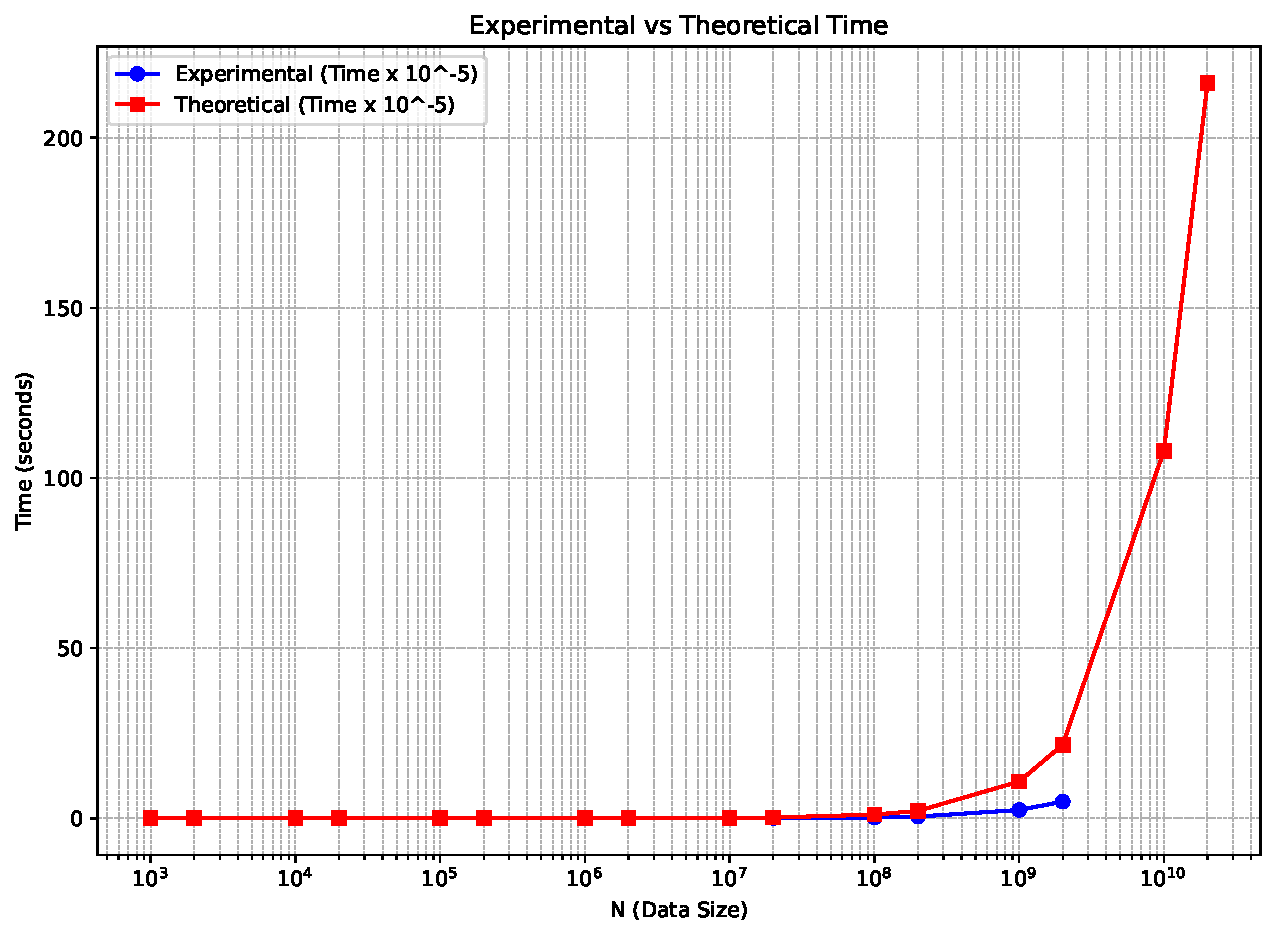
\includegraphics[width=0.85\textwidth]{Questions/Part4/plot.pdf}
    \label{fig:time_plot}
\end{figure}

\newpage

To Draw the plots i used the below python script :

\vspace{1cm}

\lstinputlisting[style=pythonstyle2,inputencoding=utf8]{Questions/Part4/draw.py}

\vspace{1cm}

\begin{prettyBox}{Observation}{greenPlot}
From the plots we notice that the 4th solution takes about the same time as 3rd solution but as n grows bigger the 4th solution takes about
half time of the 3rd therefore the 4th solution is the most efficient out of all the solutions
\end{prettyBox}




\lstinputlisting[style=cstyle]{Questions/Part1/PSUM\_1.c}

\section{Transfert Du Fichier Malveillant}

\begin{center}
    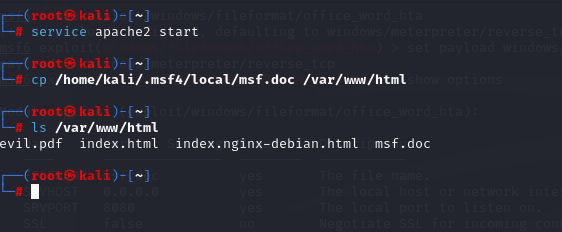
\includegraphics[width=0.8\textwidth]{Question/SC/9_kali.PNG}
\end{center}

\vspace{0.15cm}

\begin{center}
    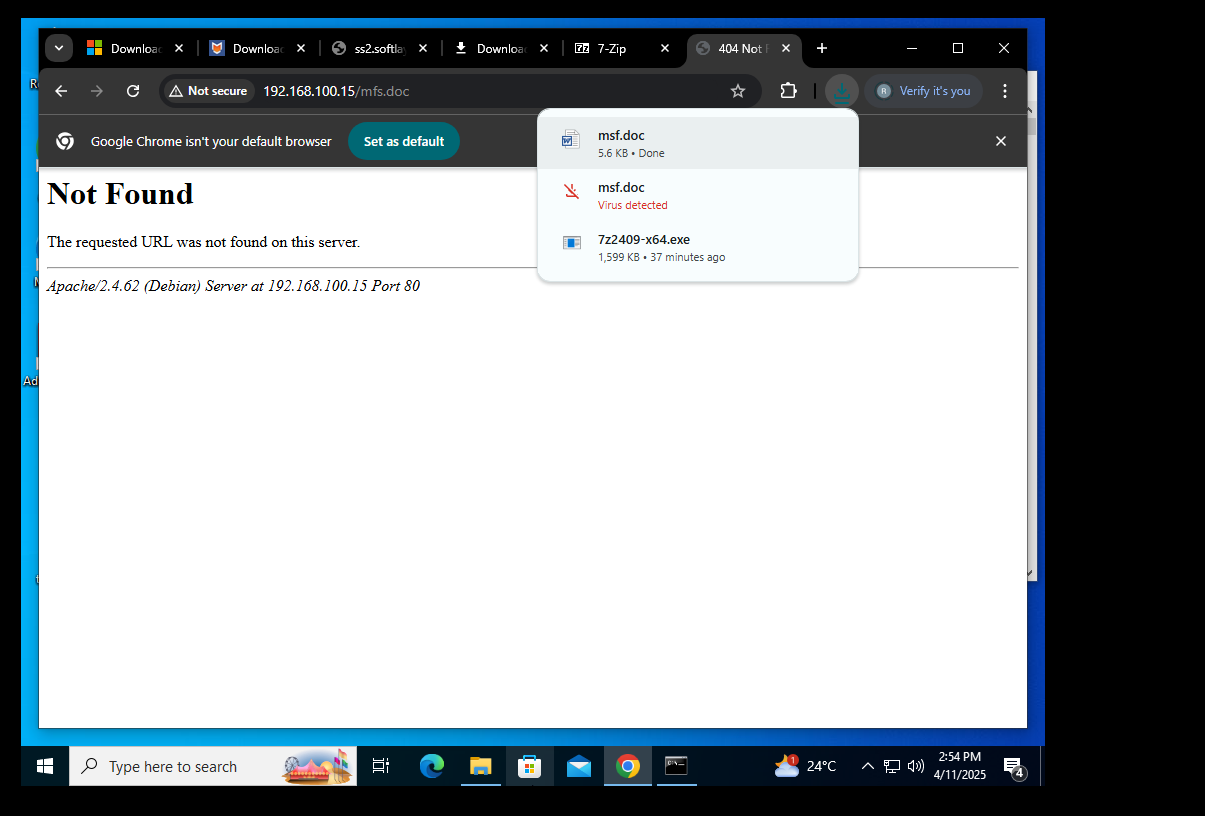
\includegraphics[width=0.6\textwidth]{Question/SC/9_win.PNG}
\end{center}

\vspace{0.15cm}

\begin{center}
    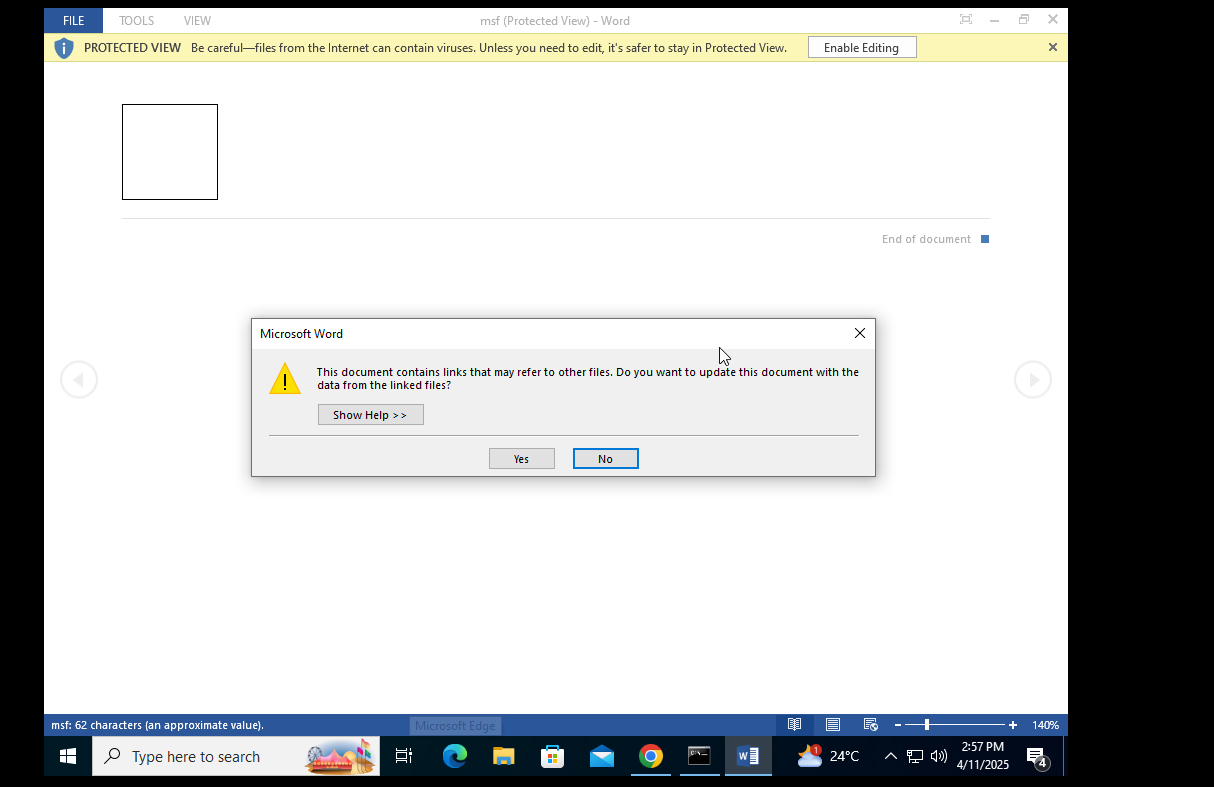
\includegraphics[width=0.6\textwidth]{Question/SC/9_3.PNG}
\end{center}


\vspace{0.35cm}

\begin{prettyBox}{Transfert de fichiers malveillants}{myblue}
\begin{itemize}
    \item On peut transférer le fichier à l'utilisateur sous un nom différent par email, lien, programme qui force l'installation, etc.
\end{itemize}
\end{prettyBox}


\end{document}
